\documentclass[output=paper]{LSP/langsci} 
\ChapterDOI{10.5281/zenodo.1291938}
\title{Disambiguate yourself: {S}upporting users in searching documents with query disambiguation suggestions}
\shorttitlerunninghead{Disambiguate yourself}

\author{Ernesto William De Luca\affiliation{University of Applied Sciences Potsdam, Germany}\lastand Christian Scheel\affiliation{Technische Universität Berlin, DAI-Labor, Berlin, Germany }}

\abstract{In this paper we present a query-oriented semantic approach and the respective architecture for supporting users in searching and browsing documents in a retrieval framework. While users are typing their queries a ``meaning-oriented'' analysis of each keystroke can provide different disambiguation suggestions (spelling correction, Named-Entity Recognition, WordNet- and Wikipedia-based suggestions) that can help users in formulating their queries for filtering relevant results. On the other hand systems can better interpret the query, because users implicitly tag the queries with the related meaning choosing the desired concept they had in mind. After the presentation of our architecture we show the results of two user studies, where users were asked to judge the support while typing their query and browsing documents. These results confirm that a semantic support is important in both cases.}
%\keywords{user modeling, semantic web, personalization, recommendation} 

\maketitle
\begin{document}
 


\section{Introduction} 
Keyword-based retrieval typically relies on keyword indexing and Boolean logic queries. These are sometimes provided with statistical methods like word frequency, where keyword lists are used to describe the content of information objects (e.g. also for finding synonyms of the query without taking into account the meaning of them). \textsc{Semantic information retrieval} is based on the cognitive view of the world, i.e. the meaning of a text (or word) depends on the conceptual relationships to objects in the world rather than to linguistic or contextual relations contained in texts or dictionaries. Sets of words, terms, etc. are mapped (in a conceptual structure) to concepts they encode. The concepts have to be identified inside the text and then classified (categorization) according to the given conceptual structure. The main types of conceptual structure are taxonomies, lexical resources (e.g. WordNet), general or domain ontologies or networks of concepts. These kind of resources have been already used for automatic disambiguation of concepts \citet{HaaLub01}. \par
Analyzing the current retrieval systems, we can state that query words are not considered in their different meanings, but only as keywords. Furthermore, they cannot deliver concept-based result lists. Because it is still difficult to understand the correlation of the search terms in a given context and documents, we believe that a semantic-based support can help in filling this gap while query typing and browsing. \par

Since the 1950s different researchers have tried to disambiguate words for different purposes such as machine translation, information retrieval and hypertext navigation, content and thematic analysis, grammatical analysis (Part-Of-Speech Tagging), speech or text processing \citet{IdeVer98}. A word is called \textsc{ambiguous} if it can be interpreted in more than one way, thus having multiple senses.  Disambiguation methods try to determine a specific sense of an ambiguous word. In general terms a word sense disambiguation process can be described as two steps, given a word $w$ that should be disambiguated:
For disambiguating word senses a variety of association methods (knowledge-driven, data-driven or corpus-based WSD) can be used \citet{IdeVer98}. 
Knowledge-based word sense disambiguation methods can be combined within semantic (or concept-based) information retrieval systems and represent one of the high-impact technologies for the next generation of \textsc{ir} systems. The search in this type of retrieval systems is based on the meaning of the searched information objects and not only on keywords in the object \citet{HaaLub01}. \par 

In this paper we present a query-oriented semantic approach and the respective architecture for supporting users in searching and browsing documents in a retrieval framework. While users are typing their queries a ``meaning-oriented'' analysis of each keystroke can provide different disambiguation suggestions (spelling correction, Named-Entity Recognition, WordNet- and Wikipedia-based suggestions) that can help users in formulating their queries for filtering relevant results. On the other hand systems can interpret the query better, because users implicitly tag the queries with the related meaning choosing the desired concept they had in mind. After the presentation of our architecture we show the results of two user studies, where users were asked to judge the support while typing their query and browsing documents. These results confirm that a semantic support is important in both cases.


\section{Supporting users with query disambiguation suggestions}
\label{sec:app_ss}
In common information retrieval there is a distinction between term-based and phrase-based queries \citet{Singhal01}. Some \textsc{ir} systems use single terms stored in the index, others also use multi-word phrases (e.g. ``Information Retrieval'') as index terms. In a similar way, in this work, users can query the index using \textsc{single word sense queries} and \textsc{multi word sense queries}. {Single word sense queries} are queries consisting of only one word that could have different meanings depending on the context they are related with. Multi word sense queries consist of the sum of different single word sense queries. Potentially, they provide more information about the context than a single word sense query. 

Auto completion of query terms is a helpful and well known feature used by many search engines. It is used to suggest word and query completions or spelling corrections. To extend this approach for suggesting word senses, there is a need for detecting possible senses in written text. If users can define their query in a meaning-oriented way, the retrieved results can be navigated easily, because they are directly related to the meaning of the search.

In the following, we describe four support approaches for query disambiguation and query typing support. These approaches are based on different resources and help to disambiguate the sense of a query from different points of view. Specifically, the goal is to improve the semantic search process; therefore several problems have to be addressed. When users mistype when writing the query, the system has to be able to give correction alternatives which is described in the following section. After this section, it is shown how to recognize named entities and suggest context-aware disambiguating concepts to retrieve only query-related documents that are semantically related.

\subsection{Spelling correction} % - an N-Gram Based Language-Independent Spell Checker
\begin{figure}
	\centering
	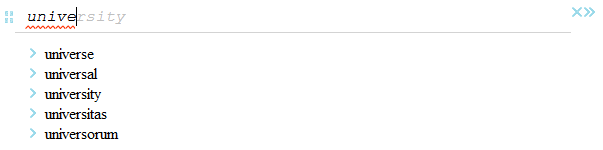
\includegraphics[width=0.8\textwidth]{figures/spelling.png}
	\caption{Spelling and auto completion suggestions}
  \label{fig:spelling}
\end{figure}

An important task for retrieving relevant documents related to the query is to identify the misspelled words and correct them for a correct interpretation. 

Auto completion and a list of term suggestions is the standard approach to support users in avoiding spelling mistakes as shown in \figref{fig:spelling}. For retrieving such suggestions, static dictionaries can be used, but for more query driven support, the selected suggestions should be related to the indexed documents. Therefore the dictionary of the index including all found senses should be used.

\subsection{Named-entity recognition (NER, Stanford)} 
Because query words used for searching documents are not only common words, but may also represent locations, organizations, time expressions, and proper nouns, a named entity recognizer (\textsc{ner}) has been added to the system, in order to support the user, if the search engine cannot disambiguate this kind of information. The Stanford \textsc{ner} \citet{FinGreMan05} can be used as a support for recognizing named entities, directing the user to the semantic search. If the user types, for example, only the name ``Java'', the \textsc{ner} should recognize the meaning of this instance and suggest more than one disambiguation possibilities (e.g. whether ``Java'' is related to the concept ``island'' or to the concept ``programming language'').

\subsection{Lexical resources (WordNet)}\label{LexRes}
In our work, we also use lexical and collaborative knowledge resources to support users in query disambiguation and semantic browsing.\par
\textsc{Lexical resources} provide linguistic information about words. This information can be represented in very diverse data structures, from simple lists to complex repositories with many types of linguistic information and relations attached to each entry, resulting in network-like structures. Lexical resources are used in Natural Language Processing (\textsc{nlp}), for example, to obtain descriptions and usage examples of different word senses. Different word senses refer to different concepts, and concepts can be distinguished from each other not only by their definitions or ``glosses'', but also by their specific relations to other concepts. Such disambiguating relations are intuitively used by humans. However, if we want to automate the process of distinguishing between word senses, we have to use resources that provide appropriate knowledge, i.e. sufficient information about the usage context of a word. One of the most important resources available for this purpose is WordNet \citet{Fel98} and its multilingual variants, including MultiWordNet \citet{Pianta02} and EuroWordNet \citet{Vossen99}.\par
WordNet \citet{Fel98} is an electronic lexical database with its theoretical design based on  psycholinguistic and computational theories of human lexical memory. It provides a list of word senses for each word, organized into synonym sets (synsets), each representing one constitutional lexicalized concept. Every synset is uniquely identified by an identifier (synsetId). It is unambiguous and carrier of exactly one meaning. Furthermore, different relations link these elements of synonym sets to semantically related terms (e.g. hypernyms, hyponyms, etc.). All related terms are also represented as synset entries. These synsets also contain descriptions of nouns, verbs, adjectives, and adverbs. With this information we can describe the usage context of a word. 

\subsection{Collaborative knowledge resources (Wikipedia)}\label{KnoRes}
The most well-known \textsc{collaborative knowledge resource} is Wikipedia\footnote{\url{http://en.wikipedia.org/wiki/Wikipedia}}. It contains 16 million articles that have been written collaboratively by volunteers and can be edited by anyone with access to the site. It is the largest online encyclopedia which provides linked and partially annotated data and descriptive information. Based on the evaluation of articles types (e.g. disambiguation pages, category articles) and the analysis of templates (e.g. info boxes) even semantic knowledge can be extracted. A popular project aiming to provide structured information from Wikipedia is \textsc{DB}pedia \citet{dbpedia}.


\section{Building sense folders for disambiguating query terms} \label{SFOverw}
As already discussed in the previous section, users can be supported with semantic information for disambiguating search terms. The semantic-based approach we presented in \citet{delNue06c} is used to simplify the search process by providing users with explicit information about ambiguities enabling them to easily retrieve the subset of documents they are looking for. In the following, we shortly describe the purpose of the \textit{sense folder approach}, defining the concept of a \textit{sense folder}, and providing an overview of the system architecture. A detailed overview of the approach is given \citet{del08book}.

\subsection{Sense folder definition} \label{SFdef}
The Sense Folder is an abstract concept that models the contextual information describing one meaning of a query word. More formally: Given a query term $q$, a sense folder is a container (prototype vector) that includes all selected linguistic information (linguistic context) of one sense of the query term retrieved from the different resources described above.\par 

In this work, we dynamically create Sense Folders based on every single query term (single word sense) selected by the users. It means that every word sense of a given term chosen is retrieved by the Sense Folder Engine and information is obtained by retrieving the related meaning from the resources explained in \sectref{sec:app_ss}. 


\subsection{System architecture} \label{SysArchit}
In order to support users in formulating queries, we decided to develop a system architecture that is able to handle two major use cases: on the one hand the system should help users in specifying an information need by using context-aware disambiguation suggestions (retrieved from different resources). On the other hand the system should support users in searching relevant information using context information implicitly retrieved by learned queries (e.g. queries that have already been typed by other users and being relevant for the given user context).
%In this section we have chosen two example queries to illustrate both use cases. It is shown which user event triggers which system response.


\figref{fig_SFArchi} gives an overview of the system architecture (and the related disambiguation process). The process starts after the user submits different query words through a user interface. For instance, every time the user types a query word (e.g. the term ``chair''), he/she will get some disambiguation suggestions (as shown in \figref{fig_SemSearchChair}) by the system. These can help him/her to better describe his/her information need. For every word contained in the query different pre-processing steps (e.g. spelling correction, named entity recognition) or semantic annotation steps (e.g. WordNet or Wikipedia annotation) can be applied and stored in Sense Folders (\textsc{sf}). All the terms are explicitly chosen by the user and describe this semantic vector \textsc{sf} that will be used to match and retrieve documents related to the query \citet{DeL10}.\par

\begin{figure} 
	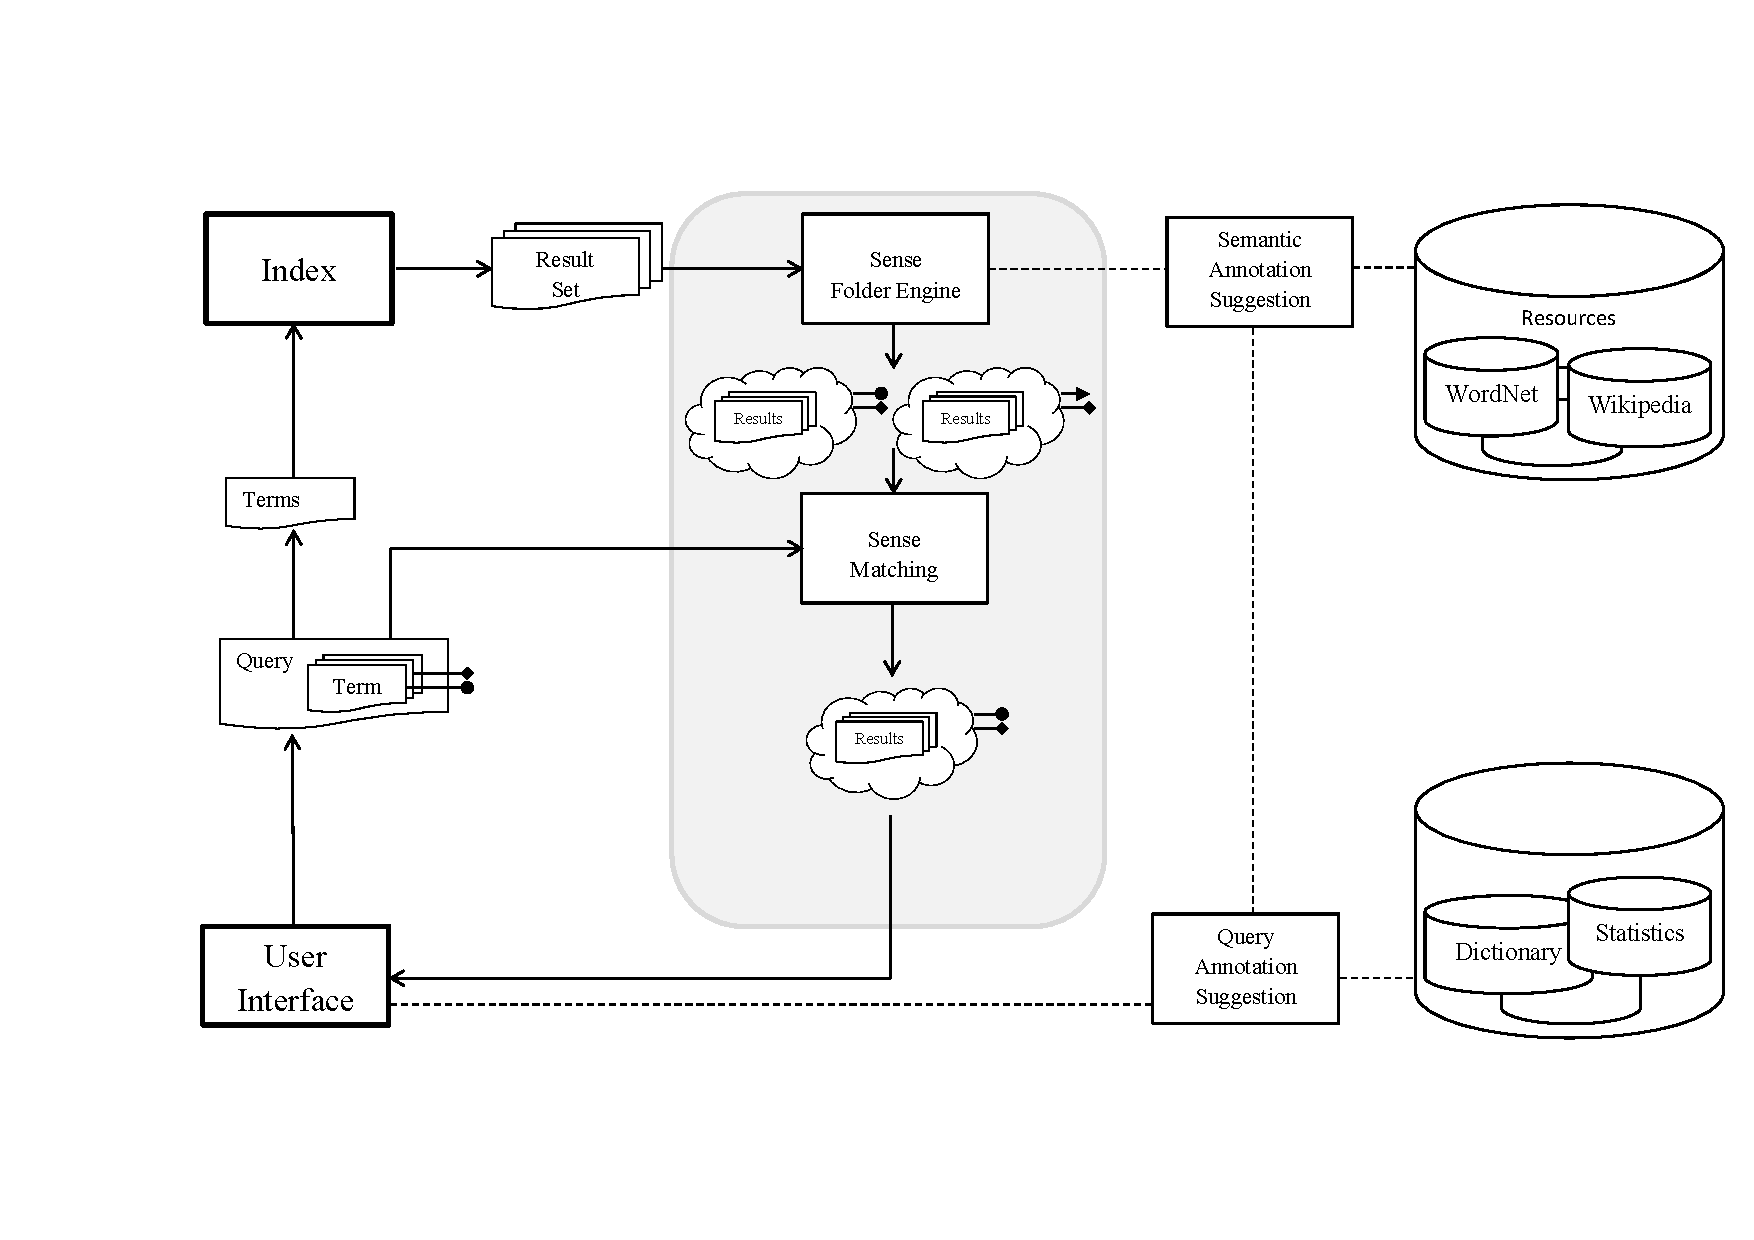
\includegraphics[width=0.5\textwidth, angle=270]{figures/sf_approach.pdf}
	\caption{System architecture: Sense Folder approach view}
	%\caption{Overview of the Sense Folder (SF) and Clustering (CL) classification process.}
	\label{fig_SFArchi}
\end{figure} 

During the query analysis, query annotation suggestions are given by the system and the user can decide to accept one of the suggested annotations in order to improve the context in which the query terms define the documents to be retrieved.\par

After the query has been processed, the users' keywords are simultaneously sent to the search engine and to the \textit{sense folder engine}. While documents are retrieved, pre-processed and indexed, for every search term the different meanings of a term  and the related linguistic relations are retrieved from the different available resource. For instance, \figref{fig_RecAnnChair} presents an example of using linguistic relations retrieved from WordNet in order to semantically annotate every term. Every query term can be expanded with words defining the context for each of its meanings, thus forming the above defined.  
Based on all words included in the relations, semantic prototype vectors (Sense Folders) describing each semantic class are constructed. The use of Sense Folder can be helpful in order to classify or cluster similar documents and present only the relevant subset to the user \citet{del08book}.

\begin{figure}[p!]
	\centering
	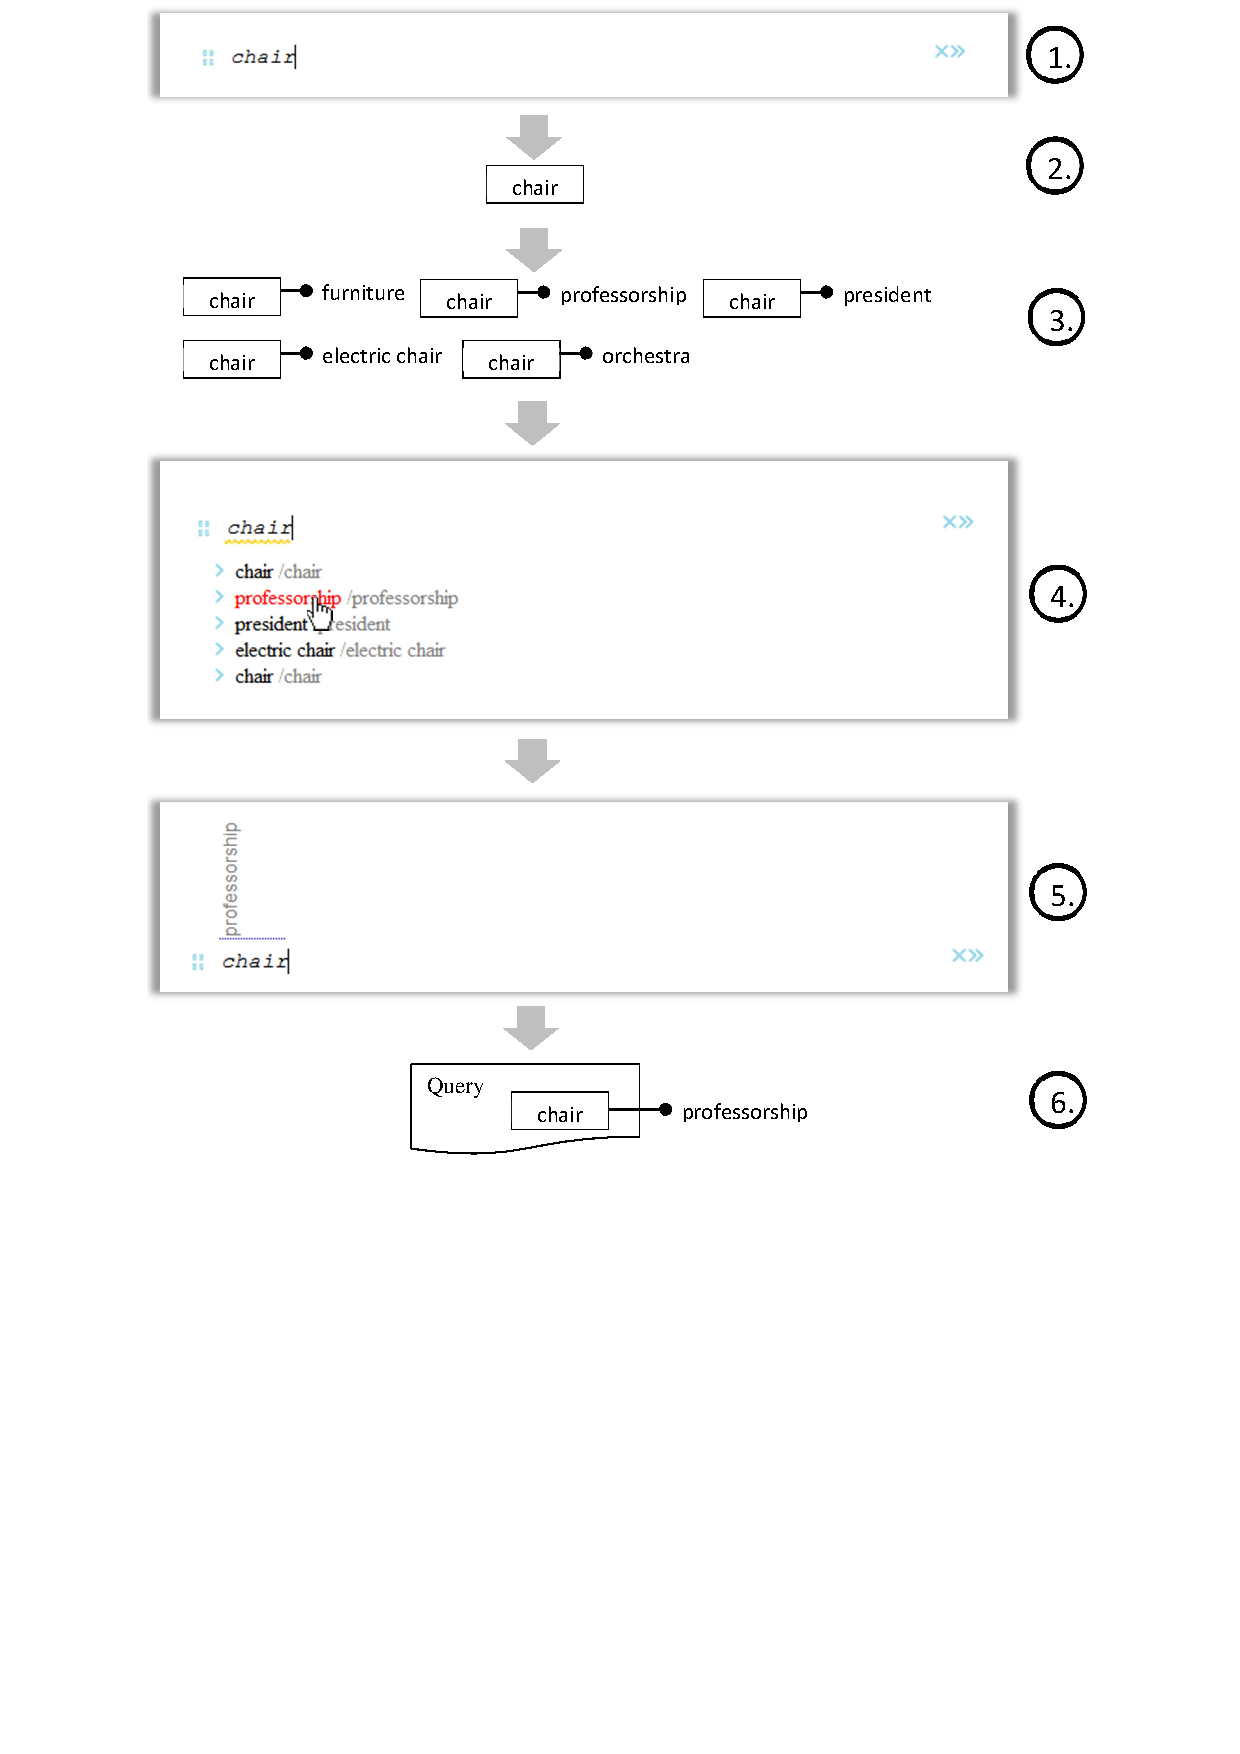
\includegraphics[width=0.8\textwidth]{figures/use_case_annotation_recommendation.pdf}
	\begin{flushleft}
    \begin{enumerate}\setlength{\parskip}{-5pt}
    	\item Event: User stops typing
    	\item Internal representation of query terms
    	\item Annotated candidates are created by the annotation suggestion module
    	\item Event: User selects the proper sense
    	\item Interface changes to visualize selection
    	\item Internal representation of annotated query term.
    \end{enumerate}
  \end{flushleft}
	\caption{Interaction between user and the retrieval system. Semantic (WordNet) annotation example for the noun collocation of the term ``chair''.}
	\label{fig_RecAnnChair}
\end{figure}

\begin{figure}[p!]
	\centering
	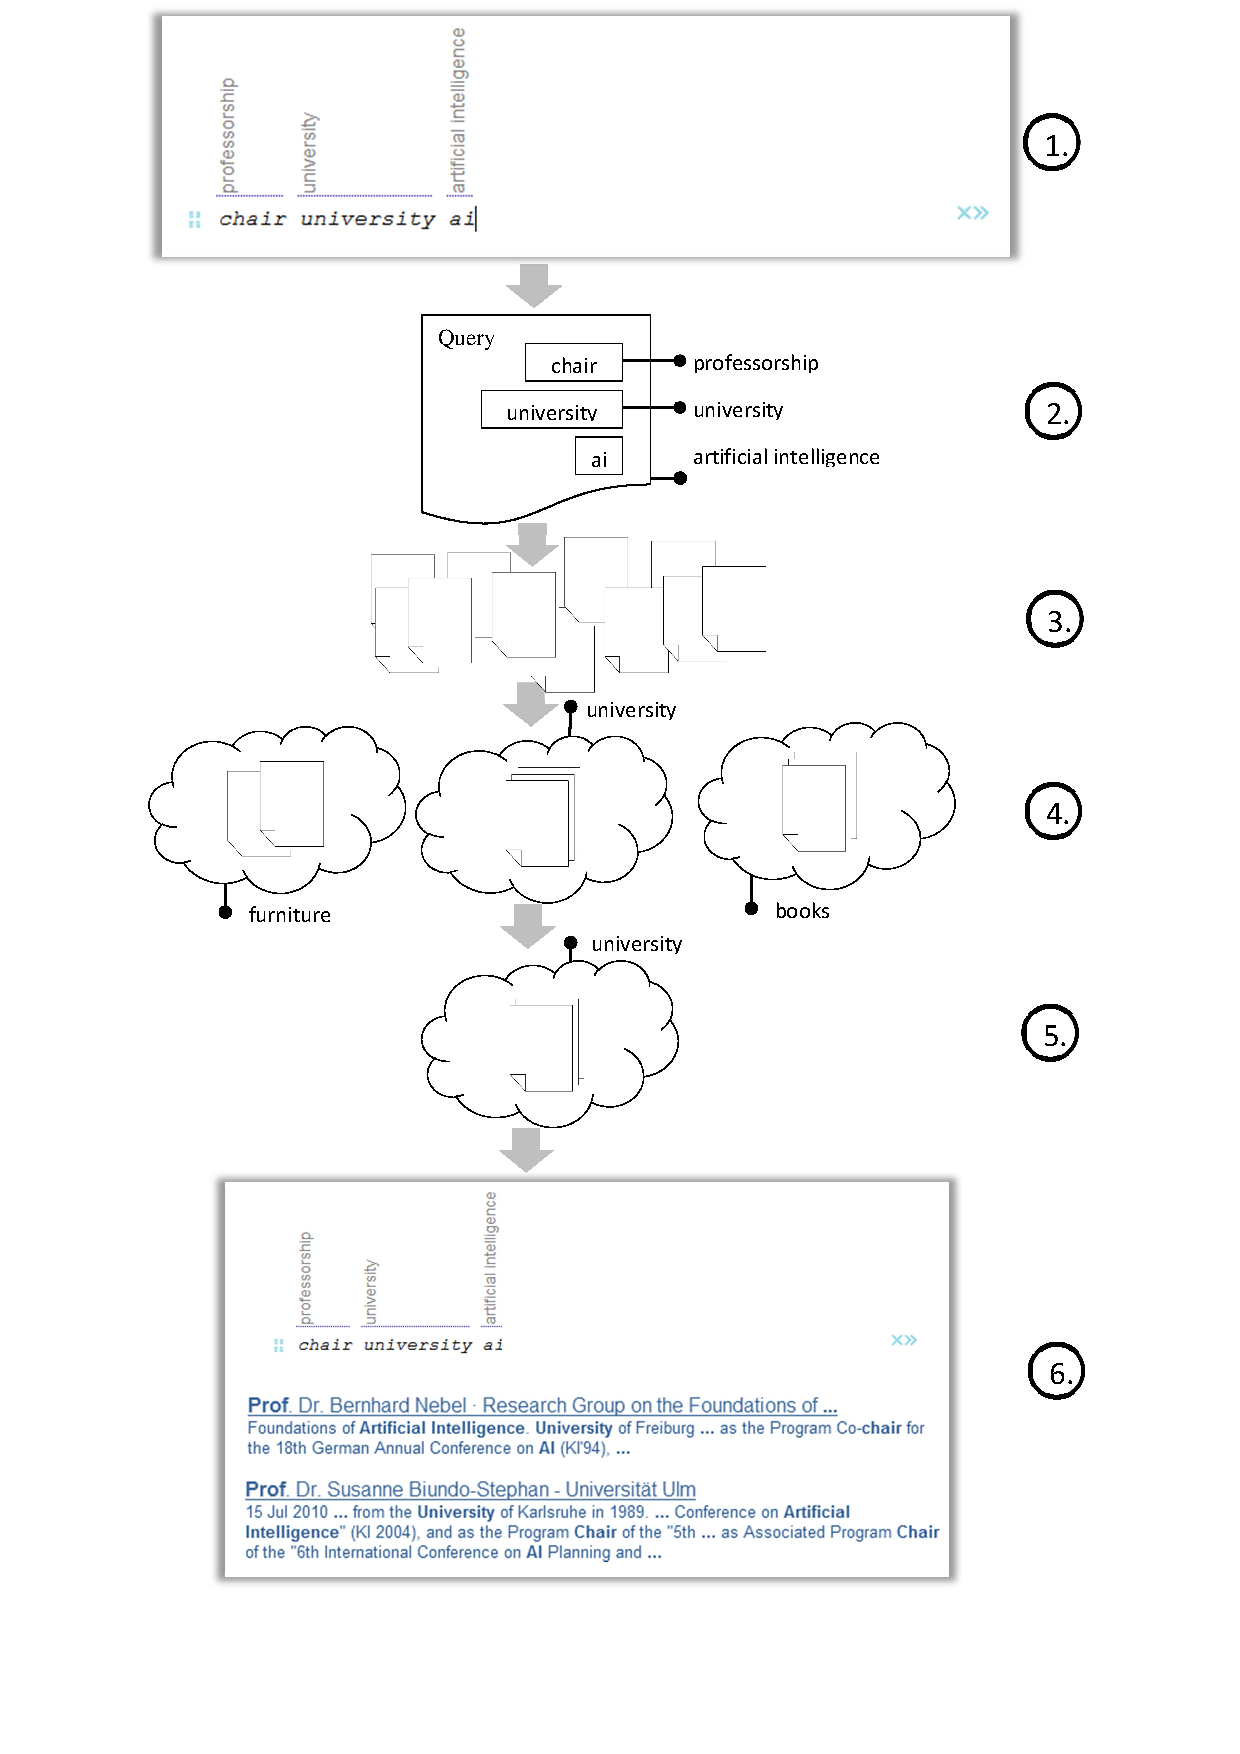
\includegraphics[width=0.6\textwidth]{figures/use_case_search.pdf}
  \begin{flushleft}
    \begin{enumerate}\setlength{\parskip}{-5pt}
    	\item Event: User starts search, after annotating the query terms
    	\item Internal representation of query: each term is connected to a Wordnet sense \textsc{id}
    	\item Based on the terms an index returns results
    	\item The sense folder architecture groups result by their meaning.
    	\item For given senses in the query, the best matching sense folder is chosen to be the result set.
    	\item Results are presented to the user.
    \end{enumerate}
  \end{flushleft}	
	\caption{Internal process of finding a result set matching user given senses}
	\label{fig_SemSearchChair}
\end{figure}

\figref{fig_RecAnnChair} shows how the system helps the user to formulate a query. The user starts his/her interaction with the system by typing the term ``chair'' which is an ambiguous term (step 1). While typing, the system suggests different senses for this term that are included in the available resources (step 2). Using WordNet \citet{Fel98}, we can observe that the system retrieves five different senses (step 3). These senses are presented to the user, raising the user's awareness for the ambiguitiy of the given term and ask to choose the word sense he/she had in mind (step 4). In this example the user decides to search for the word sense of ``chair'' that is related to the professorship concept (step 5). After this step the system knows that the user submitting this query refers to the ``chair professorship'' concept, leading to filtering the results using only this concept and providing them in the correct context of this term (step 6). 

\figref{fig_SemSearchChair} presents the retrieval process after the selection of the single word sense query explained in \figref{fig_RecAnnChair}. In this example, the user annotates the three query terms (step 1) with the context information provided by WordNet (step 2) and the system merges them for filtering relevant documents (step 3). Potential results are collected by the combination of all given word senses (step 4). Then the Sense Folder system filters these results into sets of different meanings (step 5). These meanings are compared to the given senses from the query and the best matching set is selected to be presented to the user (step 6).

\section{Evaluating the disambiguation support}\label{sec:user_study}
In order to evaluate our approaches for semantic-based query disambiguation and browsing support we conducted a user study taking into account the functionalities mentioned in the previous sections. 
The query disambiguation support functionality was tested and examined by 12 subjects (see \sectref{qoss}), while the browsing support was tested and examined by 16 subjects (see \sectref{sbs}). In the following, we summarize the results of our findings.

\subsection{User study on the query disambiguation support}\label{qoss}

In this user study we evaluated the query disambiguation support. A total of seven questions covering different aspects of typing and browsing were presented to participants.
Twelve participants were presented with suggestion results retrieved from WordNet, Wikipedia, dictionaries (for spelling correction) and Named-Entity Recognition (from the Stanford \textsc{ner}). All questions had at least one negative and one positive answer, most allowed the participants to leave short comments and motivations to their answers. The user study showed that the query typing support received overall positive opinions from the participants. In the following we summarize the results achieved:
\begin{enumerate}\sloppy
	\item Users were asked to rate the relevance of the suggestions while typing a query. Ratings are based on a one to five scale. The rating scale was as follows: indispensable (5), important (4), nice to have (3), minor (2) or irrelevant (1).  38\% said that spelling correction was `indispensable'. WordNet (53\% of the participants) and Wikipedia disambiguation pages (46\% of the participants) were seen as `nice to have' features.
	\item Similar to the first question, users were asked to rate the relevance of the suggestions while browsing the results. In this case spelling correction was a `minor' issue (23\%), while WordNet (66\% of the participants) and Wikipedia disambiguation pages (50\% of the participants) were seen as `important' features.
	\item We asked if the support was more important while typing, during the browsing or in both cases. 58\% explained that both were relevant, while 17\% preferred it while typing the query and 23\% during the browsing.
	\item Users were asked to prioritize the suggestions (spelling correction, \textsc{ner}, WordNet-based suggestions, Wikipedia-based suggestions) they would like to have while they are writing their query. On average participants wanted to have a first suggestion from a spell checker (75\%), then from WordNet (58\%), Wikipedia (50\%) disambiguation pages and Named-Entity Recognizer (50\%).
	\item Participants were asked which kind of auto completion function they would like to have as a standard. 60\% wanted to have the most frequent entities (e.g. persons, locations, and events), 23\% the most frequent words (from a dictionary) and 17\% the most frequent noun.
	\item We asked if the auto completion function should complete the word when the cursor shows its correct form, and/or the respective concept is known.  75\% would like to have this functionality, 25\% would not.
	\item Provided that the semantic-based query disambiguation functionality presented were to be integrated in the search engines of the future, we wanted to know if the users would use this possibility to narrow down the search results using the context suggestions presented. 41\% would directly use it, 83\% would use it, if they still could search in the normal way they are already comfortable with.
\end{enumerate} 

\subsection{User study on the semantic-based browsing support} \label{sbs}
In this user study we evaluated the performance of the Sense Folder approach for browsing results. A total of 9 questions covering different aspects of the Sense Folder search results presentation were asked. Sixteen participants were presented with results of the same queries from Google\footnote{\url{http://www.google.com}}, Yippi\footnote{\url{http://search.yippy.com/}} and a local deployment of the Sense Folder system (see \figref{fig_SFGUI}). Yippi was chosen because it groups similar results together into ``clouds''\footnote{\url{http://search.yippy.com/about-yippy-search}}. All questions had at least one negative and one positive answer, most allowed the participants to leave short comments and motivations to their answers.

\begin{figure}[t]
	\centering
	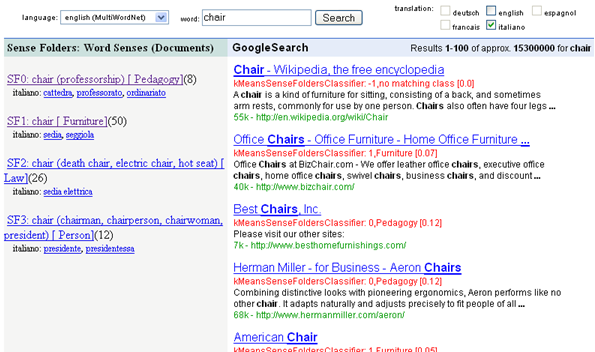
\includegraphics[width=0.6\textwidth]{figures/newSF.png}
	\caption{Using sense folders for browsing support}
	\label{fig_SFGUI}
\end{figure} 

The user study showed that the Sense Folder Approach received overall positive opinions from the participants. In the following we summarize the results achieved:

\begin{enumerate}\sloppy
	\item Users were asked to recognize the different concepts of one given word related to the search results retrieved by the search systems. Most of them (93\%) recognized between one and five concepts.
	\item Users were asked whether or not they agreed with the concepts found by the Sense Folder approach (retrieved from WordNet). 80\% said that all expected concepts were presented.
	\item The participants had to estimate the difficulty of the interaction with the Sense Folder approach. 70\% found it easy, while 17\% difficult and the remaining 13\% abstract.
	\item Users were asked to describe the differences between Goo\-gle, Yippi and the Sense Folder system. 76\% were positive to the added value of the Sense Folder annotation. The system was intuitive and supported them in disambiguating the concepts related to the query (23.5\%). The list of concepts was seen as positive (52\%). 23\% recognized that the Sense Folder system clustered documents similarly to Yippi. They also noticed that Google and Yippi only covered one dominant concept. 6\% of the participants observed that the Sense Folder system did not allow search for different media types.
	\item We asked if the Sense Folder system had been helpful and why. 81\% explained that the use of filtering by concept for the query was very positive (56\%)  and they could access information quickly and categorized by concepts. They saw an easy way of filtering results (25\%). 18\% claimed the coverage of topics was incomplete, while 6\% said they preferred to use longer queries instead.
	\item Participants were asked whether they would like to use features similar to the Sense Folder system in future search engines. 80\% were positive. They also said that the feature reduced non-relevant information (33\%), gives quick access to good results (40\%). 6\% said they preferred the Wikipedia disambiguation page due to its clustering. However, Wikipedia only presents concepts, without clustering.
	\item We asked if the participants had suggestions for improving the Sense Folder system. The majority liked it as-is. They (66\%) would however prefer a nicer user interface. This functionality  is implicitly available as documents are already filtered by concepts, by clicking on a concept, others are automatically excluded.
	\item Would they use the Sense Folder System instead of common search engine? 80\% would. 20\% of which due to the better support for finding relevant of documents, as well as the filtering of search results (60\%). The 20\%,  who chose not to use the engine, said that old habits died hard (9\%) and 11\% questioned the usability.
	\item We wanted to know which kind of search tasks users would use the Sense Folder system for. 49\% would use it for all searches, 50\% for specific searches and 6\% for none of them.
\end{enumerate}

\subsection{Evaluation summary}
Analyzing the results of our user studies we can say that semantic-based support can be very useful. 
This support during query typing and browsing is seen as positive and users would use it. However, it should not be intrusive. Different resources like WordNet and Wikipedia are seen as reasonable for semantic-based support services.\par 
While typing a query, users like to have auto completion suggestions, but rather get suggestions that can be related to the concepts they are looking for. Context exploitation is an interesting issue, when users use multi word sense queries. While typing queries users want to have one context, where the concepts are related to one another.  
This is helpful and the best matching meanings (if there is more than one word) should be presented. \par
For browsing search results in a semantic way almost all participants explained that the use of filtering by concept for the query was very positive and that they could access information quickly and categorized by concepts. They would use the Sense Folder System instead of common search engines and appreciated the added value of the Sense Folder annotation. The system supported them in disambiguating the concepts related to the query. The list of concepts was seen as positive and was desired in both user studies. \par
It is interesting to observe that many users judge spelling correction as `indispensable' while typing a query, 
but as `minor' while browsing the results. 
WordNet and Wikipedia disambiguation pages are seen as `nice to have' features
while query typing, but as `important' features for browsing.


\section{Conclusion and future work}
In this paper we presented a query-oriented semantic approach and the respective
architecture for supporting users in searching and browsing. We have shown that
a semantic-based support based on different types of suggestions (spelling
correction, Named-Entity Recognition, WordNet- and Wikipedia-based suggestions)
can help users in formulating their queries and systems in understanding the
query-related meaning. We conducted two user studies, where users were asked
to rate the support while typing their query and browsing the search results.
At the moment we are working on an agent-based extension of the system
architecture (based on the \textsc{jiac} Agent Platform, see \citealt{Hirsch2009Multi-Agent}),
where every agent is responsible for a certain resource, provides services
(e.g. spelling correction, WordNet-based suggestion, etc.) and can interact with
other agents and the user. First tests have shown promising results regarding the
flexible and reactive requirements of the proposed architecture. Together with
automatic load balancing capabilities (based on concepts like agent cloning and
mobility), we target an open dynamic environment for semantic user support.

\sloppy
\printbibliography[heading=subbibliography,notkeyword=this]

\end{document}
